\documentclass[aspectratio=169,11pt]{beamer}

\usetheme{Madrid}
\usecolortheme{default}
\setbeamertemplate{navigation symbols}{}
\setbeamertemplate{itemize items}[circle]

\usepackage[T1]{fontenc}
\usepackage[utf8]{inputenc}
\usepackage{lmodern}
\usepackage{amsmath,amssymb}
\usepackage{tikz}
\usetikzlibrary{arrows.meta,positioning,shapes.geometric}

\title{Basic Mathematics}
\subtitle{Lecture 0: Introduction}
\author{Damian Chorążkiewicz}
\date{}

\newcommand{\keyword}[1]{\textbf{#1}}

\begin{document}

\begin{frame}
  \titlepage
\end{frame}

\begin{frame}{What is this course about?}
  \centering
  \Large
  \keyword{structure}\qquad
  \keyword{space}\qquad
  \keyword{change}

  \vspace{1cm}

  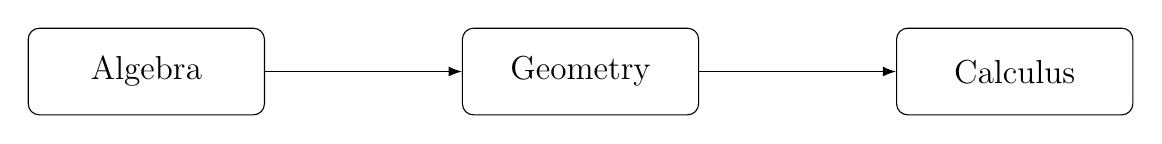
\begin{tikzpicture}[node distance=2.5cm, every node/.style={font=\large}]
    \node[draw, rounded corners, minimum width=3.0cm, minimum height=1.1cm] (alg) {Algebra};
    \node[draw, rounded corners, minimum width=3.0cm, minimum height=1.1cm, right=of alg] (geo) {Geometry};
    \node[draw, rounded corners, minimum width=3.0cm, minimum height=1.1cm, right=of geo] (cal) {Calculus};
    \draw[-{Latex}] (alg) -- (geo);
    \draw[-{Latex}] (geo) -- (cal);
  \end{tikzpicture}
\end{frame}

\begin{frame}{Not only formulas}
  \centering
  \Large
  \begin{tabular}{c@{\qquad}c@{\qquad}c}
    formula & rule & answer \\
    \Huge $\neq$ & \Huge $\neq$ & \Huge $\neq$ \\
    idea & reason & interpretation
  \end{tabular}

  \vspace{0.9cm}
  \Large
  Mathematics starts when we ask: \keyword{why?}
\end{frame}

\begin{frame}{A mathematical object}
  \centering
  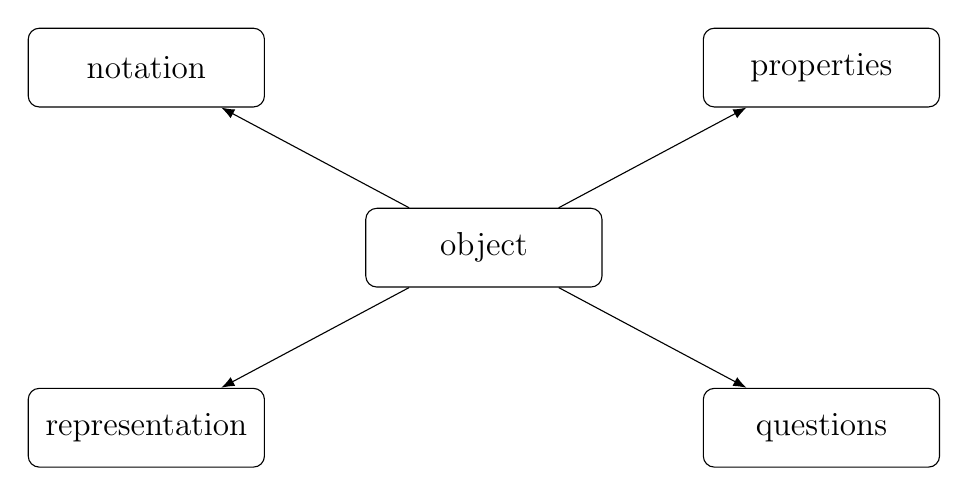
\begin{tikzpicture}[node distance=1.8cm, every node/.style={font=\large}]
    \node[draw, rounded corners, minimum width=3.0cm, minimum height=1.0cm] (obj) {object};
    \node[draw, rounded corners, minimum width=3.0cm, minimum height=1.0cm, above left=of obj] (not) {notation};
    \node[draw, rounded corners, minimum width=3.0cm, minimum height=1.0cm, above right=of obj] (prop) {properties};
    \node[draw, rounded corners, minimum width=3.0cm, minimum height=1.0cm, below left=of obj] (rep) {representation};
    \node[draw, rounded corners, minimum width=3.0cm, minimum height=1.0cm, below right=of obj] (ques) {questions};

    \draw[-{Latex}] (obj) -- (not);
    \draw[-{Latex}] (obj) -- (prop);
    \draw[-{Latex}] (obj) -- (rep);
    \draw[-{Latex}] (obj) -- (ques);
  \end{tikzpicture}

  \vspace{0.4cm}
  \Large
  First identify the object. Then choose the method.
\end{frame}

\begin{frame}{Three languages}
  \Large
  \begin{columns}[T]
    \begin{column}{0.32\textwidth}
      \centering
      \keyword{Linear algebra}

      \vspace{0.4cm}
      \[
        A x = b
      \]

      \normalsize
      vectors, matrices, systems
    \end{column}

    \begin{column}{0.32\textwidth}
      \centering
      \keyword{Analytic geometry}

      \vspace{0.4cm}
      \[
        ax+by+c=0
      \]

      \normalsize
      lines, planes, distance
    \end{column}

    \begin{column}{0.32\textwidth}
      \centering
      \keyword{Calculus}

      \vspace{0.4cm}
      \[
        f'(x),\qquad \int_a^b f(x)\,dx
      \]

      \normalsize
      change and accumulation
    \end{column}
  \end{columns}
\end{frame}

\begin{frame}{What should we ask?}
  \Large
  \begin{columns}[T]
    \begin{column}{0.48\textwidth}
      \begin{itemize}
        \item What is known?
        \item What is unknown?
        \item What is fixed?
        \item What can vary?
      \end{itemize}
    \end{column}
    \begin{column}{0.48\textwidth}
      \begin{itemize}
        \item What is the object?
        \item What is the structure?
        \item Which step is allowed?
        \item What does the result mean?
      \end{itemize}
    \end{column}
  \end{columns}
\end{frame}

\begin{frame}{A problem is not only an answer}
  \centering
  \Large
  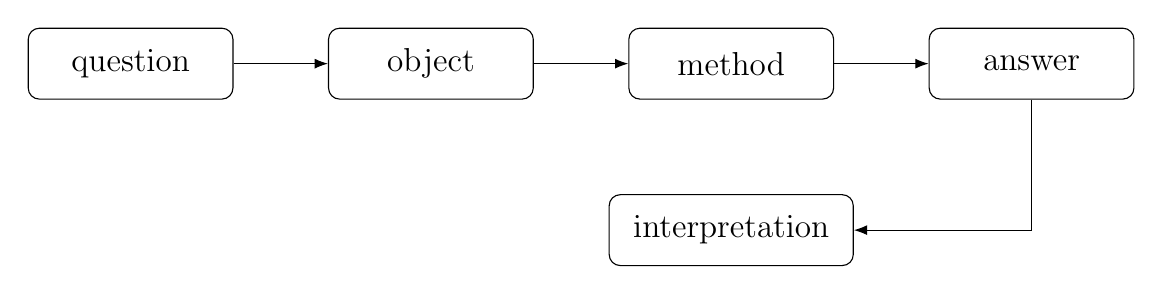
\begin{tikzpicture}[node distance=1.2cm, every node/.style={font=\large}]
    \node[draw, rounded corners, minimum width=2.6cm, minimum height=0.9cm] (q) {question};
    \node[draw, rounded corners, minimum width=2.6cm, minimum height=0.9cm, right=of q] (o) {object};
    \node[draw, rounded corners, minimum width=2.6cm, minimum height=0.9cm, right=of o] (m) {method};
    \node[draw, rounded corners, minimum width=2.6cm, minimum height=0.9cm, right=of m] (a) {answer};
    \node[draw, rounded corners, minimum width=3.1cm, minimum height=0.9cm, below=of m] (i) {interpretation};

    \draw[-{Latex}] (q) -- (o);
    \draw[-{Latex}] (o) -- (m);
    \draw[-{Latex}] (m) -- (a);
    \draw[-{Latex}] (a) |- (i);
  \end{tikzpicture}
\end{frame}

\begin{frame}{One idea, many forms}
  \centering
  \Large
  \[
    \text{algebraic} \quad \longleftrightarrow \quad
    \text{geometric} \quad \longleftrightarrow \quad
    \text{conceptual}
  \]

  \vspace{0.8cm}

  \begin{columns}
    \begin{column}{0.3\textwidth}
      \centering
      \[
        2x+3=7
      \]
    \end{column}
    \begin{column}{0.3\textwidth}
      \centering
      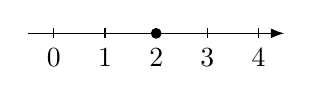
\begin{tikzpicture}[scale=0.65]
        \draw[-{Latex}] (-0.5,0) -- (4.5,0);
        \foreach \x in {0,1,2,3,4} \draw (\x,0.1) -- (\x,-0.1) node[below] {\x};
        \fill (2,0) circle (3pt);
      \end{tikzpicture}
    \end{column}
    \begin{column}{0.3\textwidth}
      \centering
      balance\\[0.2cm]
      transformation
    \end{column}
  \end{columns}
\end{frame}

\begin{frame}{How to use the PDF}
  \Large
  \begin{columns}[T]
    \begin{column}{0.46\textwidth}
      \centering
      \keyword{Slides}

      \vspace{0.4cm}
      map of the lecture\\
      ideas, formulas, examples
    \end{column}

    \begin{column}{0.46\textwidth}
      \centering
      \keyword{Notes}

      \vspace{0.4cm}
      full explanations\\
      definitions, details, reasoning
    \end{column}
  \end{columns}

  \vspace{0.9cm}
  \centering
  \Large
  Learn from the notes. Use slides to follow the lecture.
\end{frame}

\begin{frame}{Course map}
  \small
  \begin{columns}[T]
    \begin{column}{0.48\textwidth}
      \begin{itemize}
        \item Matrices
        \item Determinants
        \item Matrix inversion
        \item Systems of linear equations
        \item Vectors and coordinates
        \item Lines and planes
      \end{itemize}
    \end{column}
    \begin{column}{0.48\textwidth}
      \begin{itemize}
        \item Sequences and functions
        \item Limits and continuity
        \item Derivatives
        \item Integrals
        \item Applications of calculus
        \item Problem sets
      \end{itemize}
    \end{column}
  \end{columns}
\end{frame}

\begin{frame}{Main habit}
  \centering
  \Huge
  Ask good questions.

  \vspace{0.8cm}
  \Large
  Then compute.
\end{frame}

\end{document}
